\section{ASCbase::Prot\-Lig\-Score\-Parameters Class Reference}
\label{classASCbase_1_1ProtLigScoreParameters}\index{ASCbase::ProtLigScoreParameters@{ASCbase::ProtLigScoreParameters}}
{\tt \#include $<$Prot\-Lig\-Score\-Parameters.H$>$}

Inheritance diagram for ASCbase::Prot\-Lig\-Score\-Parameters::\begin{figure}[H]
\begin{center}
\leavevmode
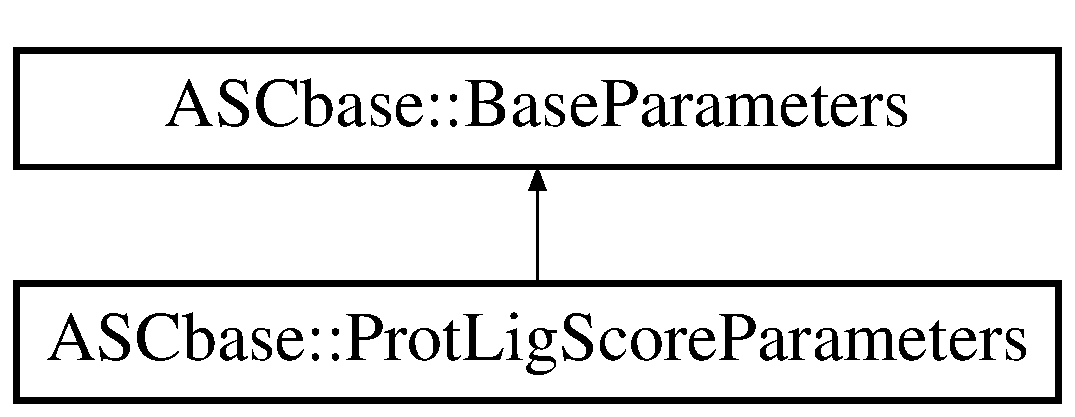
\includegraphics[height=2cm]{classASCbase_1_1ProtLigScoreParameters}
\end{center}
\end{figure}
\subsection*{Public Types}
\begin{CompactItemize}
\item 
\textbf{PRINT\_\-VERSION} = 1\label{classASCbase_1_1ProtLigScoreParameters_b7a9a2b023394c378461bd68df038bd29305d63d54f96f7ee778ef05392a7dab}

\item 
\textbf{PRINT\_\-HELP}\label{classASCbase_1_1ProtLigScoreParameters_b7a9a2b023394c378461bd68df038bd21075878cd4751c0b277fd4bc7d447435}

\item 
\textbf{BUILD\_\-INTERACTIONS\_\-TABLE}\label{classASCbase_1_1ProtLigScoreParameters_b7a9a2b023394c378461bd68df038bd291556765acaf9b14a740324aa7f42dcc}

\item 
\textbf{PRINT\_\-INTERACTIONS}\label{classASCbase_1_1ProtLigScoreParameters_b7a9a2b023394c378461bd68df038bd2fe1c72651287d18338539baf44f75cc8}

\item 
enum \textbf{popt\_\-args\_\-t} \{ \textbf{PRINT\_\-VERSION} =  1, 
\textbf{PRINT\_\-HELP}, 
\textbf{BUILD\_\-INTERACTIONS\_\-TABLE}, 
\textbf{PRINT\_\-INTERACTIONS}
 \}
\end{CompactItemize}
\subsection*{Public Member Functions}
\begin{CompactItemize}
\item 
\bf{Prot\-Lig\-Score\-Parameters} ()\label{classASCbase_1_1ProtLigScoreParameters_1d7c25c9061b1997ec8774cab0fe6ce5}

\begin{CompactList}\small\item\em To be used by the ASCbase\-Py score.parameters module. \item\end{CompactList}\item 
\bf{Prot\-Lig\-Score\-Parameters} (const int argc, const char $\ast$$\ast$argv)\label{classASCbase_1_1ProtLigScoreParameters_f8279eb37256fd5b6433900ac1ca8cab}

\begin{CompactList}\small\item\em Set the score parameters using the values in argv. \item\end{CompactList}\end{CompactItemize}
\subsection*{Public Attributes}
\begin{CompactItemize}
\item 
std::string \textbf{prot\_\-fname}\label{classASCbase_1_1ProtLigScoreParameters_d73e199c8788c4f367b7c0a246e00223}

\item 
std::string \textbf{lig\_\-fname}\label{classASCbase_1_1ProtLigScoreParameters_c6f884bad30d7e98f0fb5245dbd4d93e}

\item 
std::string \textbf{lig\_\-list\_\-fname}\label{classASCbase_1_1ProtLigScoreParameters_98f587548a6a1561b9291bfc778d5085}

\item 
bool \textbf{build\_\-interact\_\-tbl}\label{classASCbase_1_1ProtLigScoreParameters_20387a9ca9a836688d34d4e68c009632}

\item 
bool \textbf{print\_\-interactions}\label{classASCbase_1_1ProtLigScoreParameters_6d07515b95e1a858c129c8d2e6e1b5ea}

\end{CompactItemize}
\subsection*{Private Member Functions}
\begin{CompactItemize}
\item 
void \bf{init} ()
\item 
status\_\-t \bf{get\_\-opts} (const int argc, const char $\ast$$\ast$argv)
\begin{CompactList}\small\item\em Given the command line arguments, parse them using the popt library. \item\end{CompactList}\item 
status\_\-t \bf{verify\_\-parameters} ()
\begin{CompactList}\small\item\em Simple verification of command line parameters. \item\end{CompactList}\end{CompactItemize}
\subsection*{Static Private Attributes}
\begin{CompactItemize}
\item 
static const std::string \bf{A\_\-fname} = \char`\"{}Prot\-Lig\-Score\-Parameters.C\char`\"{}\label{classASCbase_1_1ProtLigScoreParameters_fa12c92a4a3e4952fd98edace796988a}

\begin{CompactList}\small\item\em Name of source file. \item\end{CompactList}\end{CompactItemize}


\subsection{Detailed Description}
A data class (public members) used to hide the details, from the main application source, needed to get the parameters. 



\subsection{Member Function Documentation}
\index{ASCbase::ProtLigScoreParameters@{ASCbase::Prot\-Lig\-Score\-Parameters}!get_opts@{get\_\-opts}}
\index{get_opts@{get\_\-opts}!ASCbase::ProtLigScoreParameters@{ASCbase::Prot\-Lig\-Score\-Parameters}}
\subsubsection{\setlength{\rightskip}{0pt plus 5cm}Base\-Parameters::status\_\-t Prot\-Lig\-Score\-Parameters::get\_\-opts (const int {\em argc}, const char $\ast$$\ast$ {\em argv})\hspace{0.3cm}{\tt  [private]}}\label{classASCbase_1_1ProtLigScoreParameters_586a96295f8218894484a4e67a903ece}


Given the command line arguments, parse them using the popt library. 

\begin{Desc}
\item[Parameters:]
\begin{description}
\item[{\em argc}]Number of command line arguments \item[{\em argv}]Array of C-style strings holding the command line arguments \end{description}
\end{Desc}
\begin{Desc}
\item[Returns:]True if parsed successfully and may continue, else false \end{Desc}
\index{ASCbase::ProtLigScoreParameters@{ASCbase::Prot\-Lig\-Score\-Parameters}!init@{init}}
\index{init@{init}!ASCbase::ProtLigScoreParameters@{ASCbase::Prot\-Lig\-Score\-Parameters}}
\subsubsection{\setlength{\rightskip}{0pt plus 5cm}void Prot\-Lig\-Score\-Parameters::init ()\hspace{0.3cm}{\tt  [private]}}\label{classASCbase_1_1ProtLigScoreParameters_71e62166bebd8b6192f7910fe3e30acb}


Initialize the class variables to standard nondefined values (such as NULL). \index{ASCbase::ProtLigScoreParameters@{ASCbase::Prot\-Lig\-Score\-Parameters}!verify_parameters@{verify\_\-parameters}}
\index{verify_parameters@{verify\_\-parameters}!ASCbase::ProtLigScoreParameters@{ASCbase::Prot\-Lig\-Score\-Parameters}}
\subsubsection{\setlength{\rightskip}{0pt plus 5cm}Base\-Parameters::status\_\-t Prot\-Lig\-Score\-Parameters::verify\_\-parameters ()\hspace{0.3cm}{\tt  [private]}}\label{classASCbase_1_1ProtLigScoreParameters_84006aef52335c65ce3c9e41eca9282d}


Simple verification of command line parameters. 

\begin{Desc}
\item[Returns:]False implies unsafe to proceed, otherwise should be OK \end{Desc}


The documentation for this class was generated from the following files:\begin{CompactItemize}
\item 
Prot\-Lig\-Score\-Parameters.H\item 
Prot\-Lig\-Score\-Parameters.C\end{CompactItemize}
